
\chapter{Background}


\section{System emulation}

% TODO: add footnote explaining that emulation and simulation will be used interchangebly
% TODO: please for the love of GOD refactor/proofread this section
System emulation is a technique of modeling and imitating the hardware of one system on another system. The range of emulation depends on the use case; some emulators, such as Wine \cite{Wine}
or QEMU in KVM mode \cite{QemuKVM}, only emulate system-level calls, executing the rest of the application natively. Another example of emulation is software like VirtualBox \cite{VirtualBox}, VMWare \cite{VMWareWorkstation}, or Microsoft
Hyper-V \cite{hyperv}, which uses host processor virtualization extensions to run the guest operating system in a supervised environment, allowing for more separation between the guest software.
More advanced emulators, such as the Renode framework \cite{Renode}, can emulate the entire platform, including processors and peripherals of another architecture. Another notable example of
such an emulator is QEMU's system mode emulation \cite{Qemu} and Intel Simics \cite{simics}.

Emulation software has become a crucial part of developing modern-day software and hardware. It finds uses in a variety of fields of software world, starting from enabling cloud
services providers with secure, reproducible, and isolated execution environments. This task is mainly handled by the level one and two hypervisors such as VMWare or Hyper-V.
Another use for emulators is the usage in continuous integration and delivery systems, where Kernel Virtual Machines (KVM), such as QEMU KVM, are widely used to aid in deploying
so-called "runners", that execute testing and deployment software in a manageable and scalable manner. Yet another scenario where emulation greatly enhances workflow is the
development of embedded/edge devices. Emulation software allows for the development of software for non-PC platforms - such as microcontrollers, SBCs or FPGA devices - without the
need for physical hardware. This decoupling has become important as development teams have grown larger and larger. This streamlines the embedded software development process by
further aligning it with classical software development practices. Emulation solutions provide first-class features such as reproducible CI pipelines, code coverage results and
other tools that have been taken for granted in the desktop development.
%

\section{Caches and memory hierarchies}

% TODO: some about how computers work here
% XXX: or maybe not?

\subsection{Role of caches in system performance}

Caching is a mechanism used to temporarily store data, that is likely to be accessed again in a (often smaller) storage medium, with a higher throughput, lower latency or higher availability,
reducing the time and resources required to retrieve it from the primary storage source. This work will cover the topic of \textit{CPU Caches}, but the general concept can be applied across
various levels of computing systems and applications.
For example, web developers use caching to store copies of web pages and other resources in storage closer to the user, by either using the browser cache, or by using the content delivery networks. % XXX: fix
Caches are also commonly used in the backend development, for example by storing the results of expensive operations - such as database queries or computationally intensive operations -
allowing for a faster access on subsequent requests. Another place where caches are used are operating systems, where caches are frequently used for storing the contents and metadata of % XXX: rewrite, this feels like a 12yo wrote it (whole paragraph)
the filesystem \cite{linuxfscache}, considerably reducing access time when the applications and services request a file.

\subsection{Overview of memory hierarchy} \label{sec:memhier}

\begin{center}
	\centering
	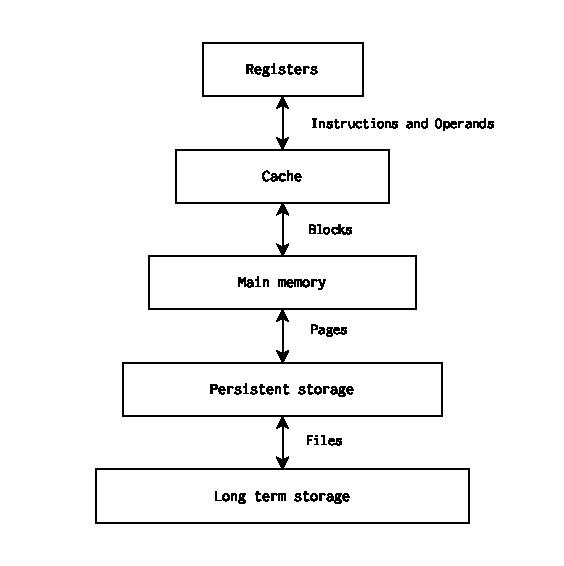
\includegraphics[width=0.75\textwidth]{figures/02-background/memhier.pdf}
	\captionof{figure}{Memory hierarchy}
	\label{fig:memhier}
\end{center}


\noindent In the context of computer organization and design, the memory hierarchy is a concept that divides computer storage mediums into a hierarchy based on a storage capacity and response time
\cite{oldbooksmarthead}. The memory hierarchy influences performance in computer architecture, impacts algorithm efficiency, and affects lower level programming constructs that rely on data locality.

\begin{itemize} % TODO: NASTY: citations for EVERYTHING here, I'm putting a ballpark figures here! marking as nasty as Im 100% sure that backing this up will be a _major_ pain in the ass
	\item \textbf{Registers:} are the smallest and the fastest storage locations within the memory hierarchy. They are located directly at the CPU core, and their access speed and capacity depends on the processor
		architecture, but typically, they can store up to 100s of bytes, and the access time is less than a nanosecond (usually not more than one CPU cycle).
	\item \textbf{Cache:} is a small, fast memory unit located very close (in the case of L2 caches) to the CPU core, or directly next to it (L1 and TLB). They are usually multi-level,
		can store from 10s to 1000s of kilobytes, and their access time is usually in the range of 1 to 10 nanoseconds \cite{Patterson2013}.
	\item \textbf{Main memory:} commonly referred to as RAM. Typically measured in gigabytes and is responsible for holding the data and instructions that the CPU needs while executing
		applications. Access times for main memory are generally in the range of 100 to 300 nanoseconds \cite{Hamacher2011}.
	\item \textbf{Persistent storage:} includes devices like hard-drives and solid-state drives. Non-volatile, measured in terabytes. Much slower than RAM, with access times in the range of 5 to 10ms.
	\item \textbf{Long term storage:} refers to external storage solutions and archival media, such as tape drives. Access times can vary widely, in case of tape drivers it is in range of several
		seconds to minutes.
\end{itemize}

\noindent Effective utilization of the memory hierarchy can drastically improve computational efficiency, for example, by careful planning and arranging data in such way, that the
CPU won't have to access main memory as often - for example by splitting large memory chunks, into smaller blocks, that will fit into cache.
Additionally, it is important to note the exponential growth in both access times and capacities as one moves down the hierarchy; while higher levels offer lightning-fast access,
their capacity is limited, whereas lower levels provide large capacity, at the cost of significantly slower access speeds. The same trend is also evident in the cost per capacity unit: the higher
up in the memory hierarchy, the more expensive the storage becomes \cite{comparchaquant}.
%

\section{CPU caches}

As noted in (\ref{sec:memhier}), caches are small and fast memories, located near or directly on the CPU die. CPU caches have been in use since the early 1960s, with the first
implementations introduced in the \textit{Atlas 2} supercomputer \cite{oldcomputercache2} and the \textit{IBM System/360 Model 85} \cite{oldcomputercache1}. They are crucial to the
performance that we can expect from modern processors, as they greatly improve the memory access cost (time or energy). Although they are relatively small compared to main memory,
typically holding thousands of kilobytes across multiple levels, their management must be quite sophisticated to correctly determine what data should be stored. Since we cannot % XXX: 'their manaegment' - find other words
store the entire memory in the caches, we encounter the problem of \textit{cache misses} - situations where the CPU attempts to access a specific address that is not present in the
cache. To demonstrate that CPU caches are an effective solution for reducing memory access cost (in terms of time), we can use mathematical analysis involving the concepts of cache % XXX: add some more glue here, this sentence feels forced
hit rates and access times. Let's assume the following:

\begin{itemize}
    \item \textbf{Cache Hit Rate ($h$)}: The fraction of memory accesses that are completed at the cache level.
    \item \textbf{Cache Miss Rate ($m$)}: The fraction of memory accesses that are not satisfied by the cache, where $m = 1 - h$.
    \item \textbf{Cache Access Time ($T_c$)}: The time it takes to access data from the cache.
    \item \textbf{Main Memory Access Time ($T_m$)}: The time it takes to access data from the main memory when a cache miss occurs.
    \item \textbf{Average Memory Access Time (AMAT)}: The average time it takes to access memory, considering both cache hits and misses.
\end{itemize}

\noindent The AMAT can be calculated using the following formula:

\[
\text{AMAT} = h \cdot T_c + (1 - h) \cdot T_m
\]

\noindent Let's consider a practical example with typical values for a modern CPU:

\begin{itemize}
    \item \textbf{Cache Hit Rate ($h$)}: 0.95 (95\%) \cite{comparchaquant}
    \item \textbf{Cache Access Time ($T_c$)}: 5 nanoseconds \cite{Patterson2013}
    \item \textbf{Main Memory Access Time ($T_m$)}: 150 nanoseconds \cite{Hamacher2011}
\end{itemize}

\noindent Plugging these values into the AMAT formula, we get:

\[
\text{AMAT} = 0.95 \cdot 5 \, \text{ns} + (1 - 0.95) \cdot 150 \, \text{ns} = 12.25 \text{ns} % FTR: the \, is a hspace
\]

\noindent To see the benefit of using a cache, let's consider the access time without a cache. In this scenario, every memory access would require the main memory access time:

\[
\text{AMAT without cache} = T_m = 150 \, \text{ns}
\]

\noindent The performance improvement due to the cache can be calculated as the ratio of the main memory access time to the AMAT:

\[
\text{Performance Improvement} = \frac{T_m}{\text{AMAT}} = \frac{150 \, \text{ns}}{12.25 \, \text{ns}} \approx 12.25 [\cdot]
\]

\vspace{10px} \noindent To get such performance enhancements, the cache must guarantee a relatively high hit-to-miss ratio. Modern caches use a variety of solutions to achieve this, such as:

\begin{itemize}
	\item \textbf{Increasing cache size:} Larger caches can store more data, reducing the likelihood of cache misses. However, this approach does not scale well,
		as the physical space on the processor die is limited and expensive, and there are often space and power usage constraints \cite{Smith1982} \cite{Hill1989}.
	\item \textbf{Multi-level caches:} Implementing multiple levels of cache (L1, L2, L3), and splitting the data and code caches (I\$, D\$) allows for a hierarchy of storage with different
		sizes and speeds. This operates on a same principle as the memory hierarchy discussed in (\ref{sec:memhier}). The L1 cache, the smallest and fastest, handles the most frequently accessed data,
		while the larger L2 and L3 caches handle less frequently accessed data.
	\item \textbf{Improved placement and eviction policies:} Algorithms for determining where data should be placed in the cache and which data should be evicted when the cache is full
		significantly enhance cache performance. These topics are covered in the (\ref{sec:placement}) and (\ref{sec:eviction_policies}) sections.
\end{itemize}

%
\subsection{Placement policies} \label{sec:placement}
Cache placement policies determine where a specific memory block can be loaded into
the cache. The choice of placement policy influences the cache architecture and
its control logic - affecting the overall complexity and performance of the system.
Each policy involves trade-offs between speed, by the means of reducing cache misses and
thrashing, and hardware costs related to the size and design of the hardware.

\vspace{10px}
\noindent Memory and cache configuration for all examples in this section:
\begin{itemize}
	\item Memory size: 1 KiB
	\item Cache size: 32 bytes
	\item Cache block size: 4 bytes
	\item Number of lines: 8
\end{itemize}

\subsubsection{Fully associative cache}
\begin{center}
	\centering
	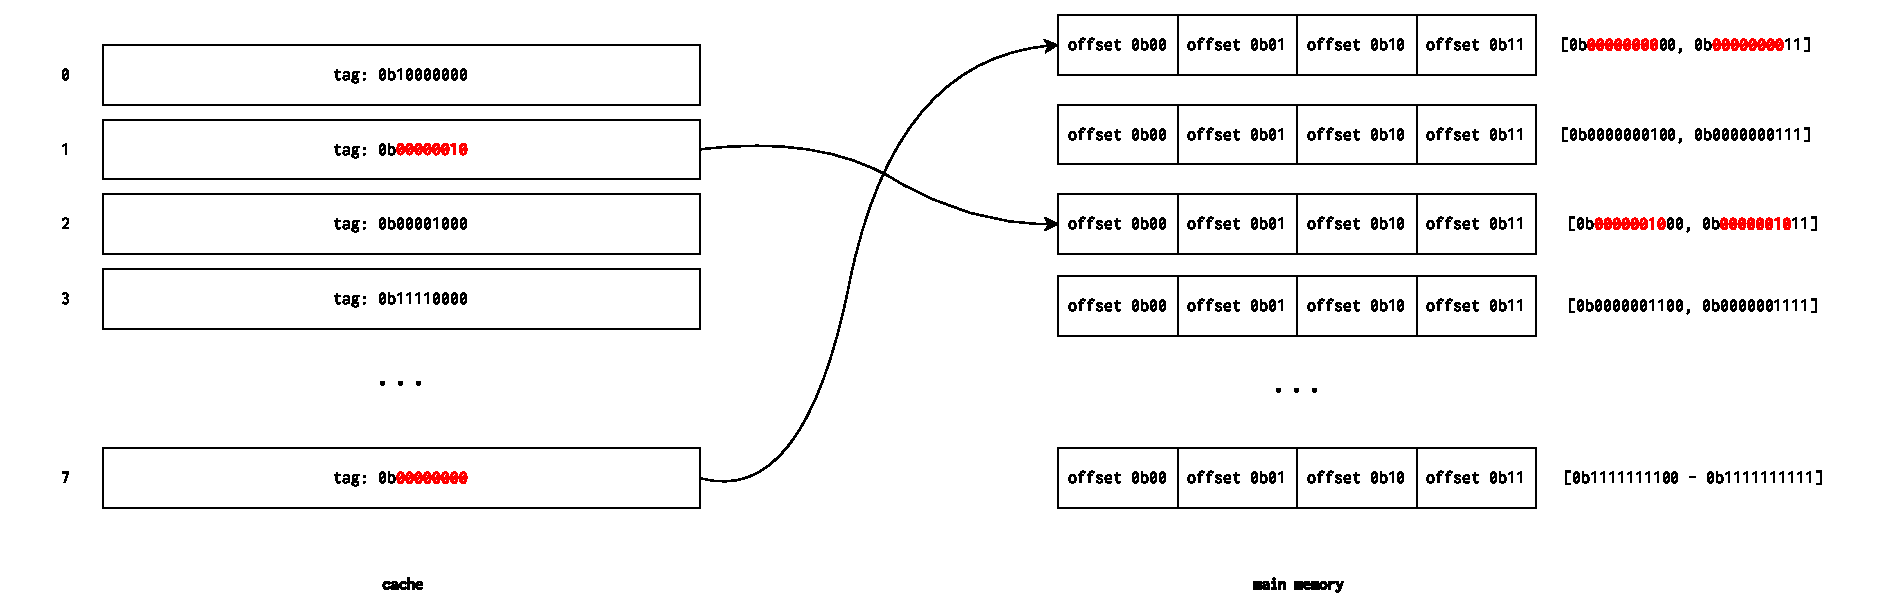
\includegraphics[width=\textwidth]{figures/02-background/full_ass_mem.pdf}
	\captionof{figure}{Visual representation of fully associative mapping}
	\label{fig:full_ass_mem}
\end{center}

\noindent In the fully associative cache each \textit{cache line} can hold a copy of \textit{any memory location}. The memory address is split into the following bit fields:

\begin{itemize}
	\item \textbf{Offset:} bits used to determine the byte to be accessed from the cache line. In this example there are two bits, that are used to address 4 bytes in the cache line.
	\item \textbf{Tag:} is used by the hardware comparator in the cache hardware design to match the address on cache request. It takes up the rest of the address, in our example 8 bits.
\end{itemize}


\noindent This configuration minimizes the chances of cache misses due to conflicts, potentially improving performance. However, this type of cache requires complex hardware for
searching and managing, as it needs to check all entries simultaneously - this means that there are needed as many comparators as there are bits in the \textit{tag} field.
This means that such implementation is unpractical and seldom used for larger caches \cite{whatevery}, this results in high power consumption and greatly increased die size.

\subsubsection{Set associative cache}
\begin{center}
	\centering
	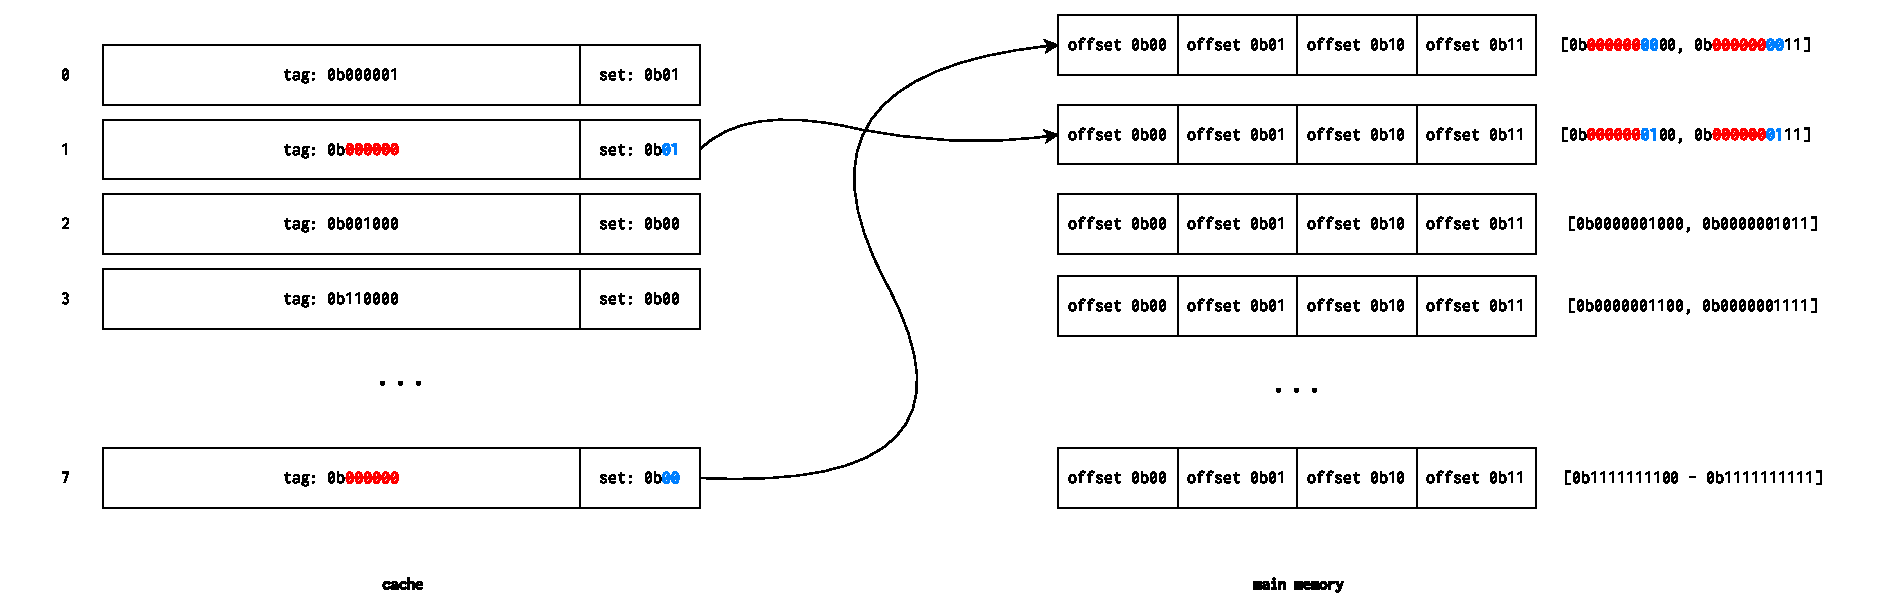
\includegraphics[width=\textwidth]{figures/02-background/set_ass_mem.pdf}
	\captionof{figure}[Visual representation of 4-way set associative mapping]{Visual representation of 4-way set associative mapping (highlighted lines sharing one set)}
	\label{fig:set_ass_mem}
\end{center}

\noindent The set associative cache introduces a concept of a \textit{set} - a collection of more than one cache line sharing the same \textit{tag}. The address is split into the following fields:

\begin{itemize}
	\item \textbf{Offset:} bits used to determine the byte to be accessed from the cache line. In this example there are two bits, that are used to address 4 bytes in the cache line.
	\item \textbf{Set:} (sometimes also called \textbf{index}) bits are used to select the cache set comparators. This example presents 4-way set associative cache - meaning that there are 4 lines
		in each set - needing 2 bits to address it.
	\item \textbf{Tag:} is used by the hardware comparator in the cache hardware design to match the address on cache request. It takes up the rest of the address, in our example 6 bits.
\end{itemize}

\noindent This configuration exchanges the flexibility of fully associative placement, for a simplified hardware model. The reduced flexibility comes from the fact that
not every memory address can be cached at the same time, let's imagine that the following addresses are loaded to the cache \texttt{0b0000\_00\_00}, \texttt{0b0001\_00\_00}, \texttt{0b0011\_00\_00}
and \texttt{0b0111\_00\_00}; all of these four lines share the same \textit{set} \texttt{0b00}, loading another address with the same set, for example \texttt{0b1000\_00\_00} would require 
an eviction of one of those lines. Eviction methods will be covered in the (\ref{sec:eviction_policies}) section. 
This tradeoff is compensated by the simplified hardware model. The only method of reducing the number of comparators, is to reduce the number of bits in the \textit{tag} field, the \textit{set}
matching can be done using simple \textit{MUX}-es \cite{whatevery}. % XXX: NASTY: i've just realised that I'm talking about comparators, but didn't explain anything about them? marking as nasty as this is a pretty big thing to explain : (
This architecture has found widespread adoption, becoming the most popular type of cache for processors in embedded devices, personal computers and high performance compute clusters
\cite{digitaldesgnandcomp} \cite{evalofcaceh}.

\subsubsection{Directly mapped cache}
\begin{center}
	\centering
	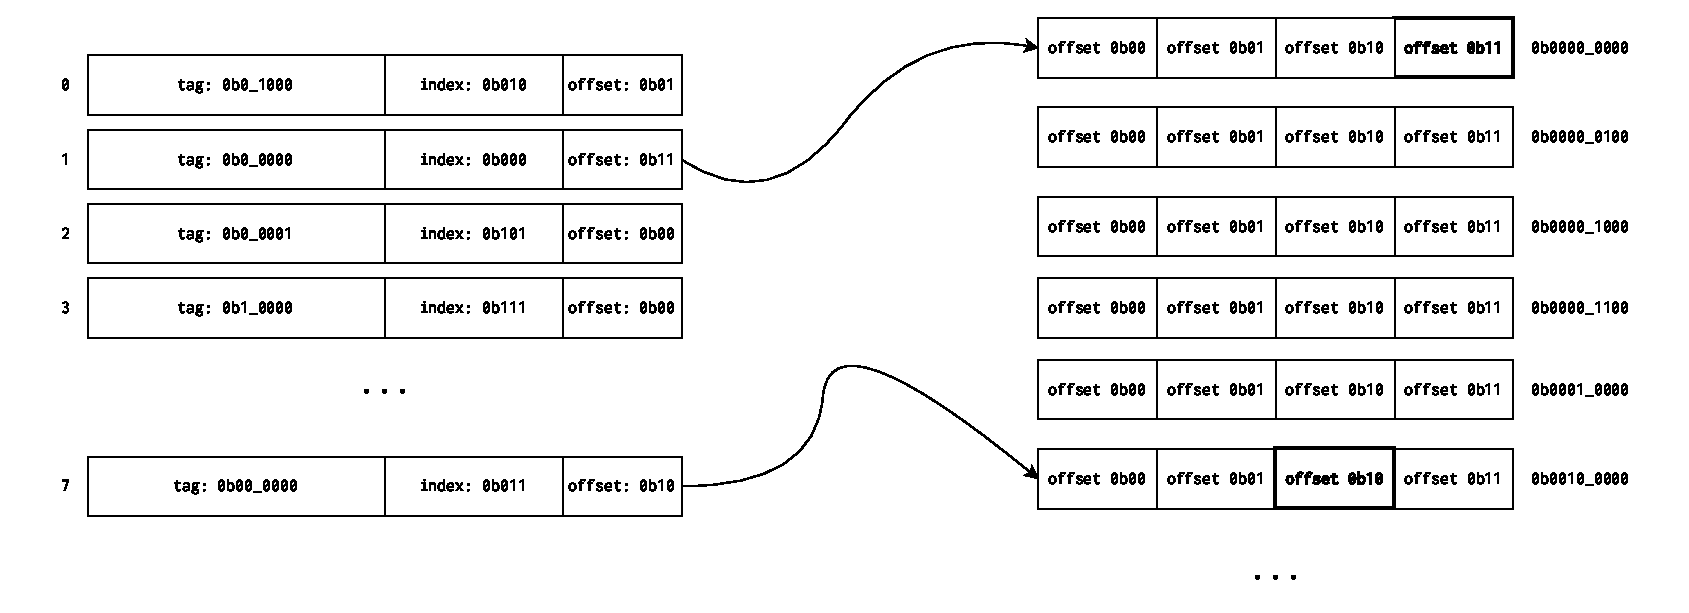
\includegraphics[width=\textwidth]{figures/02-background/dir_map_mem.pdf}
	\captionof{figure}{Visual representation of directly mapped cache}
	\label{fig:dir_map_mem}
\end{center}

\noindent In the directly mapped cache each \textit{cache line} can hold a copy of a single \textit{tag}. This policy is equivalent to the set associative cache, where the amount of sets is equal to
the number of cache lines.

\begin{itemize}
	\item \textbf{Offset:} bits used to determine the byte to be accessed from the cache line. In this example there are two bits, that are used to address 4 bytes in the cache line.
	\item \textbf{Index:}  bits are used to select the cache index comparators. Since the amount of indexes must be equal to the number of cache lines, our example uses 3 bits.
	\item \textbf{Tag:} is used by the hardware comparator in the cache hardware design to match the address on cache request. It takes up the rest of the address, in our example 5 bits.
\end{itemize}

\noindent Due to their simplicity - no need for replacement policies, and simple design, relatively small amount of supporting hardware components is needed, resulting in low power % TODO: replace design
consumption, fast and predictable accesses. Due to these characteristics fully associative caches have found usage in the TLB caches in some Intel processors \cite{whatevery}. The simplicity
comes with a drawback, they do not scale well, implementing such architecture as higher level caches, will result in lower performance when compared to another solutions. % TODO: refactor, citations


%
\subsection{Replacement policies} \label{sec:eviction_policies}
In cache design, the replacement policies describe behavior that is performed when a line needs to get \textit{evicted} from the cache memory.
The choice of replacement policy is a trade-off between cache performance and design complexity required to implement given solution. Low power
devices, such as embedded microcontrollers often opt of simple implementations, such as \textit{random eviction}, or \textit{FIFO}, as these require % TODO: add \ref to these methods
a lower amount of digital logic to select a line to evict, decreasing power consumption. High performance processors, found in PCs, servers, tablets and smartphones,
often use more advanced policies, such as \textit{LRU} and \textit{LFU}.

\subsubsection{Queue based}
% TODO(WHOLE PAR): replace 'policy' - used to often
Queue-based replacement policies use data structures such as queues to manage the replacement process. The most common queue based policy is the
\textit{First In First Out (FIFO)} policy. In this implementation the oldest cache line is replaced first. The main advantages of this policy are  % TODO: replace 'implementation'
its relative ease of implementation and predictable eviction behavior. That simplicity comes at a cost, as this policy does not guarantee optimal cache usage. The queue
based policies do not consider the frequency or recency of the data access when evicting lines, this can lead to a scenario where a data line, that has just been accessed - and due to
temporal locality - is likely to be accessed again, might get prematurely evicted from the cache, simply because it was the first loaded line.

\vspace{10px}\noindent Other queue based replacement policies include: Circular Buffer, Second Chance or Clock algorithms. % TODO: find citations

\subsubsection{Recency based}
Recency based policies prioritize data that has been accessed most recently - leveraging the concept of temporal locality - addressing one of
the main drawback of queue based policies. One of the examples of such policy is \textit{Least Recently Used (LRU)} policy. In this approach, the cache controller
keeps track of the recency of data by maintaining an ordered list of cache lines, where the most recently accessed lines are moved to the front. Due to the need of monitoring
the usage data, LRU (or other frequency based policies) require much more complex hardware designs, increasing power consumption. 

\vspace{10px}\noindent Other recency based replacement policies include: Most Recently Used, LFU with Aging or LRU-K. % TODO: find citations

\subsubsection{Frequency based}
Frequency based policies attempt to leverage the temporal locality of the memory transfers, by prioritizing the data that has been used (read) most frequently.
An example of these policies is the \textit{Least Frequently Used (LFU)}. Similarly to the recency based approaches, the cache controller tracks additional usage counters
for each line, related to the amount of times that the address has been accessed - this increases performance at the cost of increased complexity.

\vspace{10px}\noindent Other frequency based replacement policies include: Adaptive Replacement Cache, Two-Level Adaptive Replacement Cache or Least Frequently Used with Dynamic Aging. % TODO: find citations
%
\subsection{Cache coherency}

The goal of cache coherency is to maintain a consistent state between two or
more separate cache memories. This process can take place both in single-core
systems - in which the state is synchronized between two or more different levels of caches
- and in multicore processors, where the caches are kept in sync between multiple
processors.

\subsubsection{Direct memory access} \label{sec:dma}
% TODO: citations
Direct memory access, also referred to as \textit{DMA}, is a mechanism that
frees up the CPU cycles dedicated to memory operations. It is commonly used 
in one of two configurations:

\begin{itemize}
	\item \textbf{I/O to memory DMA:} In this mode, the CPU initiates the data block % TODO: back this up
		transfer, after which the DMA controller takes over to move or copy the data.
		While the transfer is ongoing, the CPU remains free to perform other operations.
		The processor receives an interrupt from the DMA controller once the transfer is complete.
		This arrangement allows for multitasking during data transactions.
	\item \textbf{Memory to memory DMA:} In this configuration the peripheral can perform memory % TODO: this too
		transfers completely independently of the CPU. This allows for high speed data transfers
		between different memory regions - often spanning multiple devices - without increasing
		the processor workload.
\end{itemize}

\noindent DMA functionality can be found in a variety of modern devices and
peripherals, starting from the relatively simple implementations found in the
UART and USART controllers, passing through more complex setups in network % TODO: cite some examples of DMA here
interfaces, and ending on high-performance computation accelerators (GPU/NPU)
and storage controllers.

\noindent In the cache coherency context, special care needs to be % TODO: cite something
taken when utilizing and implementing DMA mechanisms, the figure
(\ref{fig:dma_cache_issues}) presents the example of memory $\leftrightarrow$
cache consistency error caused by an DMA access.

\begin{center}
	\centering
	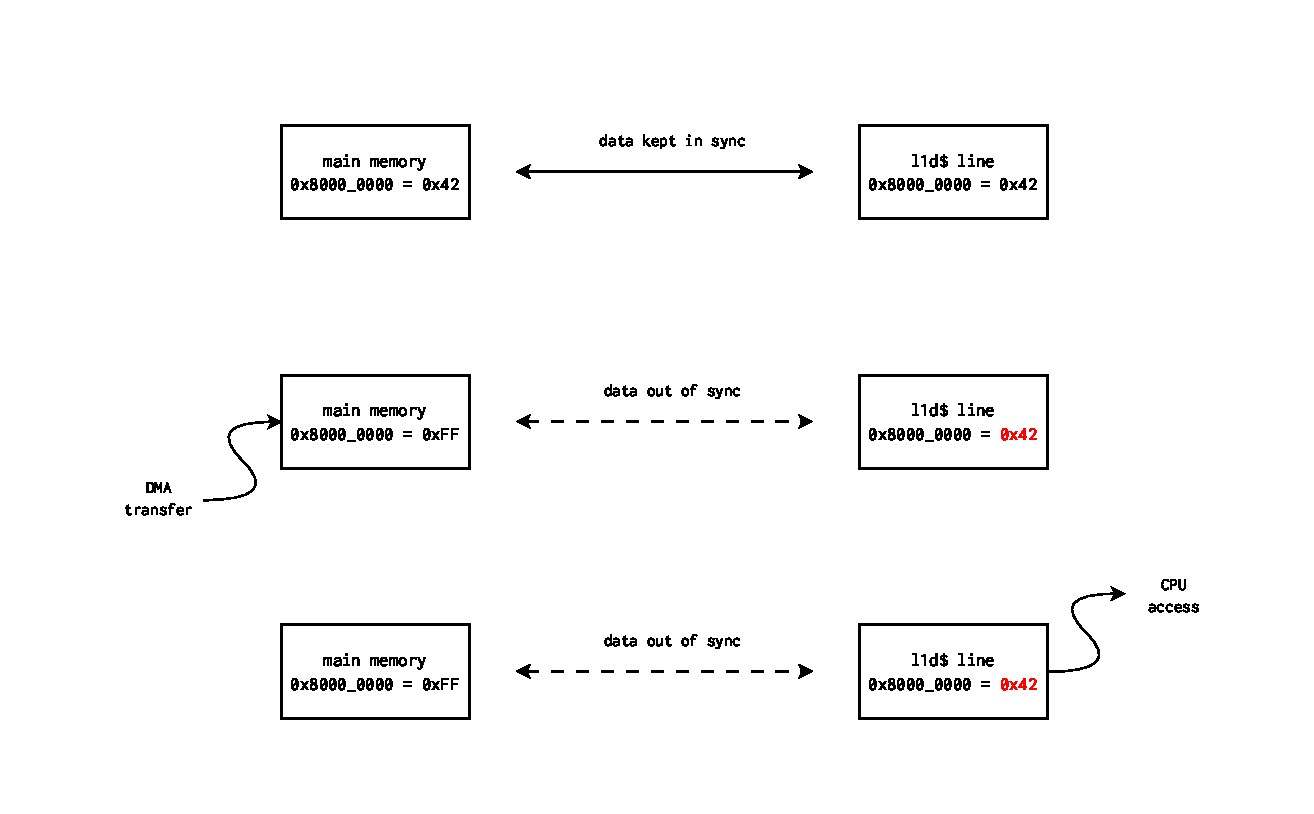
\includegraphics[width=\textwidth]{figures/02-background/dma_cache_issues.pdf}
	\captionof{figure}{Coherency error caused by a DMA transfer}
	\label{fig:dma_cache_issues}
\end{center}

\noindent This example starts off with the main memory and first level data cache - referred to as \texttt{l1d\$}, in sync.
A DMA operation updates the main memory address \texttt{0x8000\_0000} to a new value \texttt{0xFF} - The change is performed directly
in the memory, bypassing the CPU cache system. When CPU accesses this memory address, it retrieves the value from its
cache line, which has not been updated, as the DMA transfer was completely transparent for the processor.
In system design, there are two main ways to address such problems:

\begin{itemize}
	\item \textbf{Hardware approach:} \textit{bus snooping} (sometimes also referred to as\textit{bus sniffing}) is an % TODO: cite bus spoofing
		approach where an additional hardware coherency controller - called \textit{snooper} - monitors the outstanding
		transfers on the bus. When external access to a bus is detected, it sends a signal to the cache system, where the
		effected caches are either flushed, or the invalid lines are marked as \textit{dirty}. The primary advantage of this solution is the reduced
		complexity of the operating system and/or drivers, coupled with the CPU executing fewer instructions - at the cost of increased hardware complexity. % TODO: lots of 'complexity' here, refactor so it flows better
	\item \textbf{Software approach:} in designs where implementing hardware coherency solution is not possible - due to space, power or cost constraints -
		the software solutions must be used. In these cases the operating system, or the device drivers, must keep track of ongoing DMA transfers, and manually
		invoke cache invalidating and flushing instructions when necessary. While such solutions reduce the overall hardware design complexity, they add a
		runtime overhead for the processor.
\end{itemize}


\subsubsection{Symmetric multiprocessing}
% TODO: citations

In the context of CPU's, symmetric multiprocessing (or shared-memory multiprocessing) is a system architecture, where two or more \textbf{identical processors} % TODO: add a footnote that SMP implies homogeneous systems (and CITE this as this is a pretty bold statement lol)
are running \textbf{independently of each other}. In SMP systems processors share a common memory pool, allowing for data sharing and communication
between cores. Such configuration requires that multiple cores share a common bus. Some examples of such buses include \textit{Front-side bus}, \textit{Intel Ultra Path Interconnect} % TODO: add citations here (yes, I'm artifically inflating the bilbiography :))
and \textit{HyperTransport} on the x86 personal computers; examples used in embedded systems are \textit{Arm Advanced Microcontroller Bus Architecture} and \textit{SiFive TileLink}. % TODO: citation for AMBA TODO: XXX: is tilelink valid here?

One of the key benefits of SMP designs is their ability to increase performance in a scalable manner, benefiting from parallelization of workloads among multiple cores. % TODO: really please start citing this
Another advantage of such designs is the increased data throughput between multiple cores, which tend to be physically located close to each other on the silicon die.
This proximity allows for much higher bus clock frequencies, thereby increasing the maximum possible data transfer bandwidth on the shared bus. % TODO: lots of 'bus' here

In the context of cache coherency, processors in SMP systems typically share not only the main memory but also higher-level caches - such as level 2 and level 3 caches.
The contents of first level of cache are usually not shared between cores. Despite L1 being private to each core, coherence must be maintained across all cache levels. % TODO: footnote explaining cache sync vs cache cocherence
This is achieved by using various \textit{coherence protocols}, such as \textbf{MESI} (Modified, Exclusive, Shared, Invalid) and \textbf{MOESI} (Modified, Owned, Exclusive, Shared, Invalid).
This work will not cover the specific implementation details of these protocols. % XXX: nice cliffhanger ;) but rly maybe I should at least to try to put a simplified diagram 'ere?

